\chapter{Diagramok}
\thispagestyle{empty}

Diagramok segítségével grafikusan ábrázolhatjuk a
táblázatok számadatait. A diagramok automatikusan követik a
táblázat változásait. A Calc az adatok módosítását
követően újraépíti a diagramot. Többféle diagramtípus
közül választhatunk és az elkészült diagramokat utólag is
módosíthatjuk.


\section{Diagramtündér használata}

A \textbf{Beszúrás} menü vagy a \textbf{Standard} eszköztár
\textbf{Diagram} parancsával kezdhetünk hozzá a diagram
elkészítéséhez. Mindkét esetben a \textbf{Diagramtündér}
ablaka jelenik meg, ami végigvezet minket a diagram
elkészítésének négy lépésén. Megkönnyíti a diagram
létrehozását, ha a Diagramtündér indítása előtt
kijelöljük azt a tartományt vagy tartományokat, amelyekből
diagramunk felépül.

Nyissuk meg a calc01 munkafüzetet és a 4. feladat adatai alapján
készítsünk diagramot, ami a napi eladásokat mutatja.
Jelöljük ki az A3:A6, majd a Ctrl billentyűt lenyomva tartva a
D3:H6 tartományt (\ref{DiagramTartomány} ábra).

\begin{figure}[!h]
\begin{center}
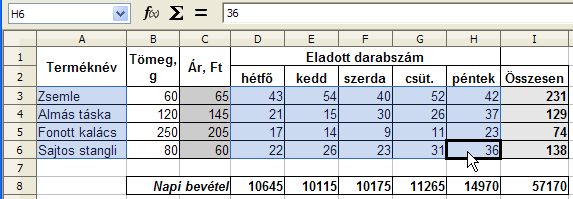
\includegraphics[width=15.159cm]{oocalcv2-img52.png}
\caption{Diagram készítése -- tartomány kijelölése}\label{DiagramTartomány}
\end{center}
\end{figure}

Indítsuk el a Diagramtündért. Az első lépésben
kiválaszthatjuk a diagram típusát és azon belül az
altípust. A számadatok típusa általában meghatározza a
választható kategóriákat. Válasszuk az \textbf{Oszlop}
diagramtípust és a \textbf{Halmozott} altípust (\ref{DiagramTípus} ábra).

\begin{figure}[!h]
\begin{center}
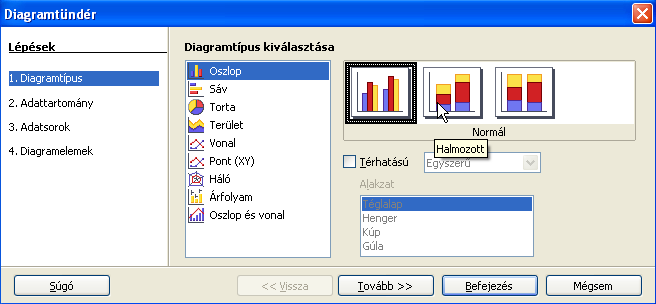
\includegraphics[width=15.999cm]{oocalcv2-img53.png}
\caption{Diagram készítése --  diagramtípusok}\label{DiagramTípus}
\end{center}
\end{figure}

A diagramtündér használata közben a munkalapon kék színnel
vannak kiemelve a kiindulási cellák, és láthatjuk az e cellák
adatai alapján létrejött, általunk választott típusú
diagramot is. Figyeljük meg, hogyan változik a diagram a normál
és a halmozott altípust választva. 

A Shift+F1 billentyűkombináció segítségével, a
Diagramtündér ablakának elemeiről részletes magyarázatot
olvashatunk, ha az egér mutatóját az adott elemre vezetjük.

A Tovább gombra kattintva a Diagramtündér második
lépése, az \textbf{Adattartomány} következik (\ref{DiagramAdat} ábra).
 Itt kijelölhetjük, vagy módosíthatjuk a diagram forrását.

\begin{figure}[!h]
\begin{center}
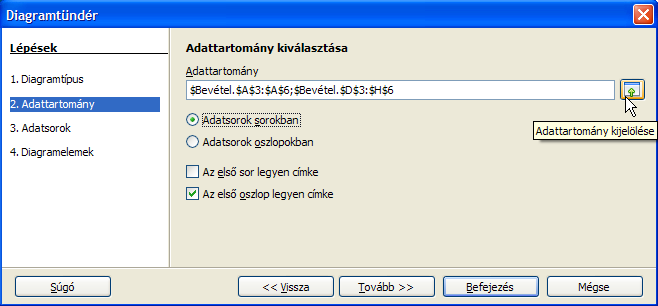
\includegraphics[width=15.999cm]{oocalcv2-img54.png}
\caption{Diagram készítése --  adattartomány}\label{DiagramAdat}
\end{center}
\end{figure}

Esetünkben az adattartomány két, pontosvesszővel
elválasztott, abszolút címzésű cellatartomány, ahol a
cellacímek előtt a munkalap nevét látjuk. Tehát a
\textbf{\$Bevétel.\$A\$3:\$A\$6} hivatkozás a Bevétel nevű
munkalap A3:A6 tartományát jelöli abszolút címzéssel. Így
hivatkozhatunk munkalapok között cellatartományokra a Calckal.

Amennyiben szükséges, hozzáadhatunk adattartományt
pontosvesszőt írva a meglévők után és az
\textbf{Adattartomány kijelölése} gombra kattintva (\aref{DiagramAdat}
ábrán az egér rá mutat). A Ctrl billentyűt lenyomva tartva
egérrel adhatunk meg további tartományokat. 

Ebben a feladatban attól függően, hogy az \textbf{Adatsorok
sorokban} vagy az \textbf{Adatsorok oszlopokban} választókapcsoló
közül melyik aktív, a diagram vízszintes tengelyére a
péksütemények nevei vagy a hét napjai kerülnek. Válasszuk
az \textbf{Adatsorok sorokban} kapcsolót.

\textbf{Az első sor legyen címke} és \textbf{Az
első}\textbf{ oszlop legyen címke} kapcsolók
automatikusan aktívak mert  a kijelölt területen az első sor
és az első oszlop cellái szöveges információt
tartalmaznak.

A következő lépés az \textbf{Adatsorok} (\ref{DiagramAdatsor} ábra).
Ebben az ablakban az adatsorok sorrendjét módosíthatjuk, és ha
szükséges, újabb adatsorokat adhatunk a diagramhoz.

\begin{figure}[!h]
\begin{center}
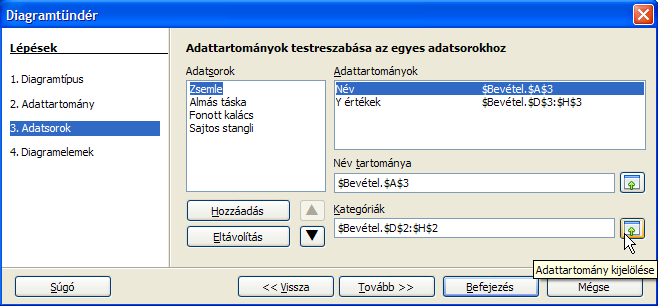
\includegraphics[width=15.499cm]{oocalcv2-img55.png}
\caption{Diagram készítése --  adatsorok}\label{DiagramAdatsor}
\end{center}
\end{figure}

Az adatsorok valamelyikét választva látjuk, hogy melyik
cellatartomány tartalmazza az adott adatsor számértékeit és
melyik cellában van az adatsor neve.

A \textbf{Kategóriák} részben látható cellatartomány a
diagramon az X tengely felirata lesz. Esetünkben a hét napjai
kerüljenek Ehhez válasszuk az \textbf{Adattartomány
kijelölése} kapcsolót és jelöljük ki a D2:H2 tartományt.

\begin{figure}[!h]
\begin{center}
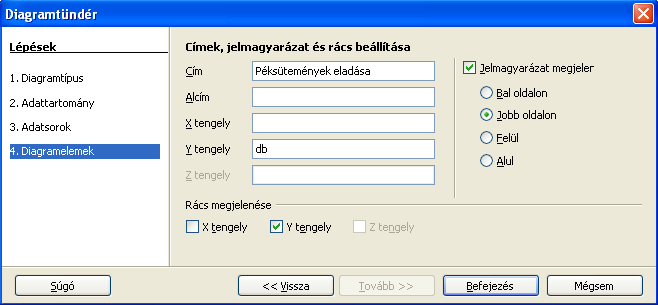
\includegraphics[width=15.499cm]{oocalcv2-img56.png}
\caption{Diagram készítése --  diagramelemek}\label{DiagramElemek}
\end{center}
\end{figure}

A diagramtündér utolsó, negyedik ablakában címet és
alcímet adhatunk a diagramnak és a tengelyeknek (\ref{DiagramElemek} ábra).
Cellahivatkozást nem adhatunk meg, a szöveget közvetlenül kell
beírni.

A jelmagyarázat tartalma a forrástartomány első sorból vagy
oszlopból, illetve az Adatsorok párbeszédpanelen megadott
tartományból áll. Diagramon belüli pozícióját
választókapcsolókkal állíthatjuk be. Megjelenítését ki
is kapcsolhatjuk, de olyan diagramoknál, amikor az adatsor
értékek tartománya több cellából áll, fontos
információt hordoz. Esetünkben a halmozott oszlopdiagram
különböző színnel jelölt elemeinek magyarázatául
szolgál.

A \textbf{Befejezés} gombra kattintva megjelenik a munkalapon a
diagram (\ref{Diagram} ábra). 

\begin{figure}[!h]
\begin{center}
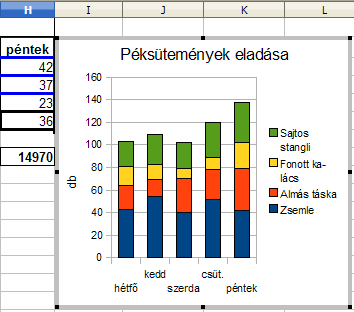
\includegraphics[width=8.364cm]{oocalcv2-img57.png}
\caption{Diagram}\label{Diagram}
\end{center}
\end{figure}

Az elkészült diagramról a péksütemények napi eladásait
olvashatjuk le. Az x tengelyen feltüntetett  napokhoz egy-egy oszlop
tartozik, amelyek magassága az eladások összegének a
darabszámát mutatja az adott napon. Az oszlop különböző
színű részekből áll, amelyek arányosak egyes termékek
napi eladásával. A színek magyarázatát a jelmagyarázatban
találjuk.

A diagram diagramszerkesztési nézetben jelent meg. Ilyenkor a
menüsor és az eszköztár is átalakul (\ref{DiagramSzerkesztés} ábra).

\begin{figure}[!h]
\begin{center}
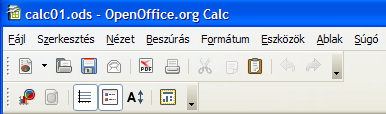
\includegraphics[width=10.211cm]{oocalcv2-img58.png}
\caption{Diagram szerkesztési menü}\label{DiagramSzerkesztés}
\end{center}
\end{figure}

A munkalapra kattintva kilépünk a diagramszerkesztési
nézetből, így módosíthatjuk a diagram  méretét és a
munkalapon elfoglalt pozícióját. 


\section{A diagram módosítása}

Az elkészült diagramot formailag, tartalmilag egyszerűen
módosíthatjuk. A diagramra kettőt kattintva
diagramszerkesztési nézetbe jutunk, ahol a gyorsmenüből (jobb
egérgomb), vagy \aref{DiagramSzerkesztés} ábrán látható menüsor és
eszköztár parancsaival módosíthatjuk azt.

A módosítandó diagramelemet kijelölve és azon kettőt
kattintva, az adott elem tulajdonságait mutató ablak jelenik meg,
ahol elvégezhetjük a szükséges módosításokat.


\section{10. feladat}
{\itshape
A 4. feladat adatai alapján készítsünk tortadiagramot, ami a
keddi eladásokat mutatja. Módosítsuk az elkészült diagramot
\aref{10-feladat} ábrának megfelelően.}

\begin{figure}[!h]
\begin{center}
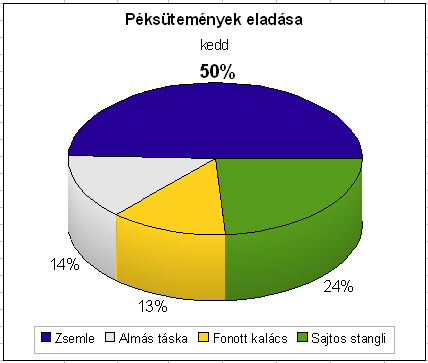
\includegraphics[width=11.324cm]{oocalcv2-img59.png}
\caption{10. feladat}\label{10-feladat}
\end{center}
\end{figure}

A diagram építését kezdjük a diagramtündér
indításával. Gyakorlásképpen az adattartományt is itt adjuk
meg. Az első lépésben válasszuk a \textbf{Torta}
diagramtípust, \textbf{Normál} altípust és kapcsoljuk be a
\textbf{Térhatású} kapcsolót is. A második lépést az
\textbf{Adattartomány kijelölése} paranccsal kezdjük és
jelöljük ki a péksütemények neveit. Ezután válasszuk
ismét az Adattartomány kijelölését, írjunk
pontosvesszőt a hivatkozás után és a Ctrl billentyűt
lenyomva tartva jelöljük ki a keddi számadatokat
(\ref{10-feladatAdattartomány} ábra).

\begin{figure}[!h]
\begin{center}
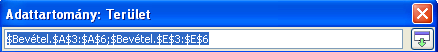
\includegraphics[width=11.589cm]{oocalcv2-img60.png}
\caption{10.  feladat --  adattartomány}\label{10-feladatAdattartomány}
\end{center}
\end{figure}

Kapcsoljuk ki \textbf{Az első sor legyen címke} kapcsolót.
Monitorunk felbontásától függően a diagramtündér ablaka
takarhatja a készülő diagramot. Az ablakot a címsávnál
fogva helyezhetjük át ideiglenesen, hogy ellenőrizhessük a
diagramot.

A harmadik ablakban semmit sem kell módosítani, kattintsunk a
tovább gombra. A negyedikben írjuk be a címet és az alcímet,
a jelmagyarázat helye legyen \textbf{Alul}.

A kész diagramot helyezzük át a munkalapon a táblázat alá
és növeljük meg a méretét. Kettős kattintással
váltsunk diagramszerkesztési nézetre és a \textbf{Formátum}
menü \textbf{Térbeli nézet} ablakának \textbf{Megjelenés}
fülén kapcsoljuk be az \textbf{Árnyalás}t és az
\textbf{Objektumszegélyek}et (\ref{10-feladatTérbeli} ábra).

\begin{figure}[!h]
\begin{center}
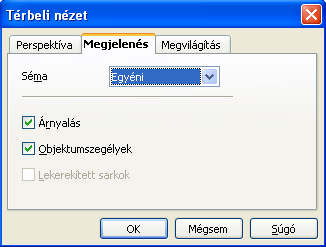
\includegraphics[width=6.636cm]{oocalcv2-img61.png}
\caption{10.  feladat --  térbeli nézet}\label{10-feladatTérbeli}
\end{center}
\end{figure}

A tortadiagram egyik adatpontjának módosításához ki kell
jelöljük azt. Kettős kattintással, a gyorsmenü
segítségével (\ref{10-feladatObjektum} ábra), vagy a \textbf{Formátum} menüpont
\textbf{Objektum tulajdonságai} ablakban válasszuk a
\textbf{Terület} fület.

\begin{figure}[!h]
\begin{center}
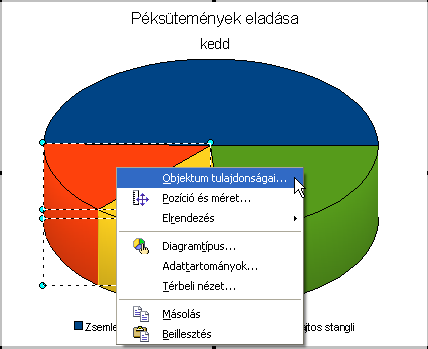
\includegraphics[width=11.324cm]{oocalcv2-img62.png}
\caption{10. feladat --  Objektum tulajdonságai}\label{10-feladatObjektum}
\end{center}
\end{figure}

\clearpage
Válasszuk a \textbf{Szín} kategóriából a \textbf{Szürke
10\%}-ot. Fekete-fehér nyomtató estén hasznos lehet a
\textbf{Vonalkázás} kategória, de választhatunk díszes
\textbf{Színátmenet}et és \textbf{Bitkép}et is.

Hasonlóképpen módosítsuk a Jelmagyarázat tulajdonságait. A
\textbf{Karakterek} fülön válasszunk 10 pt betűméretet és
Arial betűtípust. A \textbf{Szegélyek} fülön
\textbf{Folyamatos} stílust.

A diagram címének betűmérete legyen 14 pt és félkövér
formátumú.

A \textbf{Beszúrás} menüpont \textbf{Adatfeliratok} ablakában
kapcsoljuk be az adatsorok mellett a százalékérték
 megjelenítését is (\ref{10-feladatFeliratok} ábra).

\begin{figure}[!h]
\begin{center}
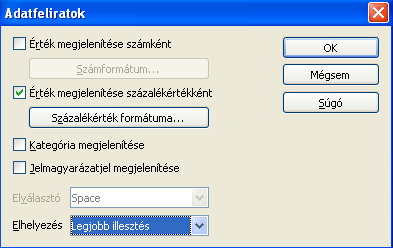
\includegraphics[width=10.398cm]{oocalcv2-img63.png}
\caption{10.  feladat --  adatfeliratok}\label{10-feladatFeliratok}
\end{center}
\end{figure}

A százalékértékek betűméretét módosítsuk 12-re, majd
a legnagyobb százalékértéket (50\%) külön is kijelölve
14-re és félkövér betűstílusra.

A diagramterületet kijelölve állítsunk be folyamatos stílusú
szegélyvonalat.


\section{Pont (XY) diagram építése}

Pont diagram segítségével értékpárokat (x, y)
ábrázolhatunk. Ez az a diagramtípus, amelyik segítségével
matematikai függvények grafikonjait is megrajzolhatjuk. 


\section[11. feladat]{11. feladat}

{\itshape
Ábrázoljuk diagramon az  $y=a+(b+x)^{2}$ függvény grafikonját
az \textbf{x} -10, -9, {\dots}, 10 értékeinél. Az \textbf{a} és
a \textbf{b} értékeket a B1, B2 cella tartalmazza.}

A diagram építéséhez először az \textbf{\textit{x}}
értékek oszlopát hozzuk létre. Írjuk az A5 cellába -10-et.
Automatikus kitöltéssel lefelé a Calc segít nekünk a
számoszlop létrehozásában (\ref{11-feladat} ábra).

\begin{figure}[!h]
\begin{center}
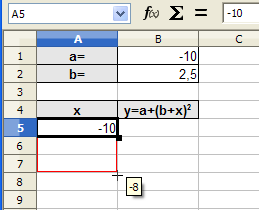
\includegraphics[width=6.851cm]{oocalcv2-img64.png}
\caption{11. feladat}\label{11-feladat}
\end{center}
\end{figure}

Az \textbf{\textit{y}} értékek kiszámításánál a képlet
=B\$1+(A5+B\$2)\^{}2 lesz, hiszen az \textit{x} értéknek
változnia kell automatikus kitöltésnél, az \textit{a} és
\textit{b} értékek pedig állandóak (64. ábra).

A diagramtípus kiválasztásánál az \textbf{Pont~(XY)} típust
és \textbf{Csak~vonalak} altípust válasszuk. A
\textbf{Sima~vonalak }kapcsoló legyen aktív. A
\textbf{Diagramelemek} ablakban a jelmagyarázatot kikapcsolhatjuk,
hiszen csak egy adatsorunk van.  A rácsot kapcsoljuk be az X
tengelyre is (\ref{11-feladatMegoldás} ábra).

\begin{figure}[!h]
\begin{center}
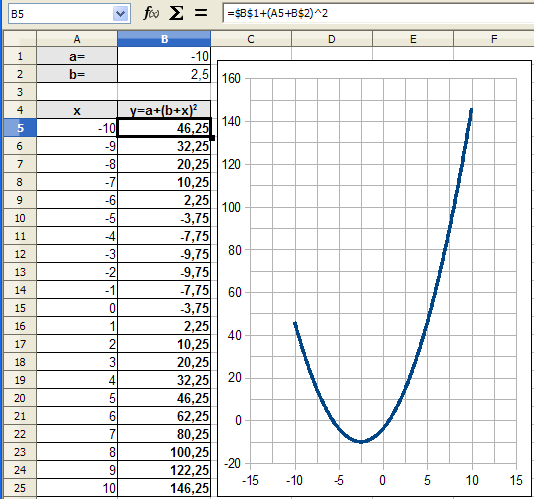
\includegraphics[width=12.458cm]{oocalcv2-img65.png}
\caption{11. feladat -- Megoldás}\label{11-feladatMegoldás}
\end{center}
\end{figure}

